\documentclass[handout]{beamer}  

%Smaller gap at between top and bottom of block when there are displayed equations
\addtobeamertemplate{block begin}{\setlength\abovedisplayskip{0pt}}
{\setlength{\belowdisplayskip}{0pt}}


\usepackage{setspace}
\linespread{1.3}
\usepackage{amssymb, amsmath, amsthm} 
\usepackage{rotating}
\usepackage{multirow}
\usepackage{graphicx}
\usepackage{synttree}
\usepackage{verbatim}
\usepackage{fancybox}
\usepackage{color}
\usepackage{tikz}
\usetikzlibrary{shapes,backgrounds}
\usepackage{hyperref}
\usetikzlibrary{trees}
\newcommand{\p}{\mathbb{P}}
\newcommand{\expect}{\mathbb{E}}


%\setbeamertemplate{blocks}[rounded][shadow=true] 
%gets rid of bottom navigation bars
\setbeamertemplate{footline}{
   \begin{beamercolorbox}[ht=4ex,leftskip=0.3cm,rightskip=0.3cm]{author in head/foot}
%    \usebeamercolor{UniBlue}
    \vspace{0.1cm}
    %\insertshorttitle \ - \insertdate 
    \hfill \insertframenumber / \inserttotalframenumber
   \end{beamercolorbox}
   \vspace*{0.1cm}
} 


%gets rid of navigation symbols
\setbeamertemplate{navigation symbols}{}


%Include or exclude the notes?
%\setbeameroption{show notes}
\setbeameroption{hide notes}

\title[Econ 103]{Economics 103 -- Statistics for Economists} 
\author[F. DiTraglia]{Francis J.\ DiTraglia}
\institute{University of Pennsylvania}
\date{Lecture 13}


\begin{document} 
%%%%%%%%%%%%%%%%%%%%%%%%%%%%%%%%%%%%%%%%

\begin{frame}[plain]
	\titlepage 
	

\end{frame} 


%%%%%%%%%%%%%%%%%%%%%%%%%%%%%%%%%%%%%%%%
\begin{frame}
\Huge \begin{center}
Continuous RVs -- Part III
\end{center}
\end{frame}
%%%%%%%%%%%%%%%%%%%%%%%%%%%%%%%%%%%%%%%%
\begin{frame}

\begin{block}{Last Time}
\begin{itemize}
	\item Expectation for Continuous RVs
	\item Normal Random Variable
	\item Linear Combination of Normal RV
	\item Areas under Normal pdfs
\end{itemize}
\end{block}

\begin{block}{Today}
	\begin{itemize}
		\item Percentiles/Quantiles for Continuous RVs
		\item Linear Combination of \emph{\alert{Several}} Normal RVs
		\item Friends of Normal Distribution
	\end{itemize}
\end{block}


\end{frame}

%%%%%%%%%%%%%%%%%%%%%%%%%%%%%%%%%%%%%%%%

\begin{frame}
\frametitle{Recall: Def.\ of Cumulative Distribution Function (CDF)}


\begin{eqnarray*}
F(x_0) &\equiv& P(X \leq x_0) \\ \\
		&=& \int_{-\infty}^{x_0} f(x)\; dx \mbox{ for Continuous RVs}
\end{eqnarray*}


\end{frame}
%%%%%%%%%%%%%%%%%%%%%%%%%%%%%%%%%%%%%%%%
\begin{frame}
\frametitle{Percentiles/Quantiles for Continuous RVs}
\begin{block}{Quantile Function $Q(p)$ is the inverse of CDF $F(x_0)$}
Plug in a probability $p$, get out the value of $x_0$ such that $F(x_0)=p$
\end{block}
$$Q(p) = F^{-1}(p)$$
\pause
In other words:
	$$Q(p) = \mbox{the value of } x_0 \mbox{ such that } \int_{-\infty}^{x_0} f(x) \; dx = p$$
	
\begin{alertblock}{Inverse exists as long as $F(x_0)$ is \emph{strictly increasing}.} \end{alertblock}	
	
\end{frame}
%%%%%%%%%%%%%%%%%%%%%%%%%%%%%%%%%%%%%%%%
\begin{frame}
\frametitle{Example: Median}
The median of a continuous random variable is $Q(0.5)$, i.e.\ the value of $x_0$ such that 
	$$\int_{-\infty}^{x_0} f(x)\; dx = 1/2$$
\end{frame}
%%%%%%%%%%%%%%%%%%%%%%%%%%%%%%%%%%%%%%%%
\begin{frame}
\frametitle{What is the median of a standard normal RV?\hfill 
\includegraphics[scale = 0.05]{./images/clicker}}
\pause
By symmetry, $Q(0.5) = 0$. R command: \texttt{qnorm()}
\begin{center}
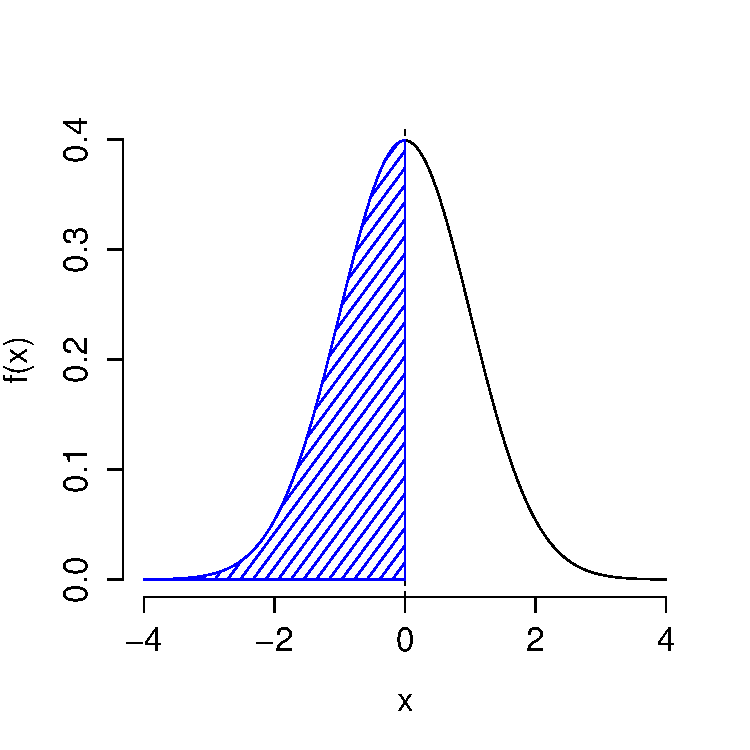
\includegraphics[scale = 0.6]{./images/normal_median}
\end{center}
\end{frame}
%%%%%%%%%%%%%%%%%%%%%%%%%%%%%%%%%%%%%%%%
\begin{frame}
\frametitle{90th Percentile of a Standard Normal}
\texttt{qnorm(0.9)}$\approx 1.28$
\begin{center}
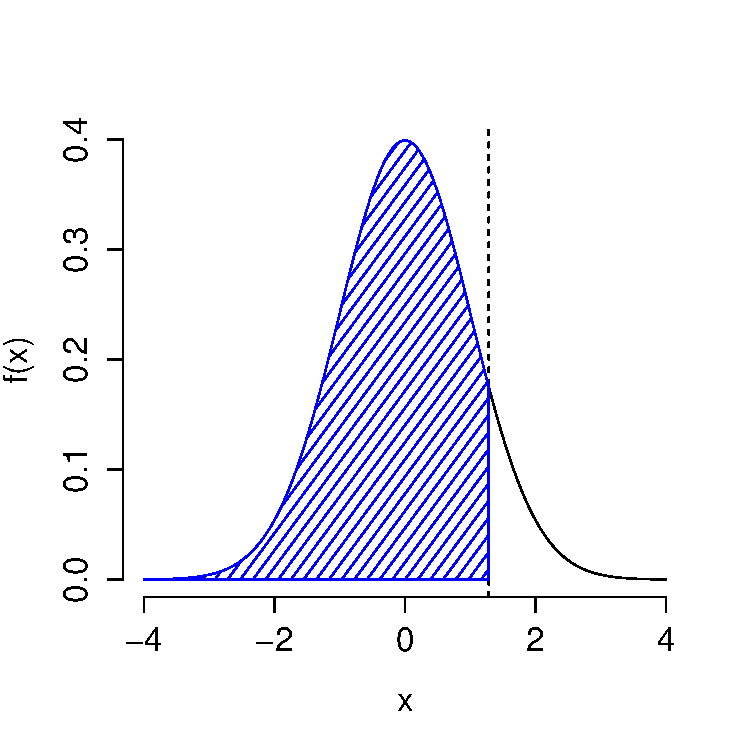
\includegraphics[scale = 0.6]{./images/normal90}
\end{center}
\end{frame}
%%%%%%%%%%%%%%%%%%%%%%%%%%%%%%%%%%%%%%%%

\begin{frame}
\frametitle{Using Quantile Function to find Symmetric Intervals}
Suppose $X$ is a standard normal RV. What is the value of $c$ such that $P(-c \leq X\leq c ) = 0.5$?
\begin{center}
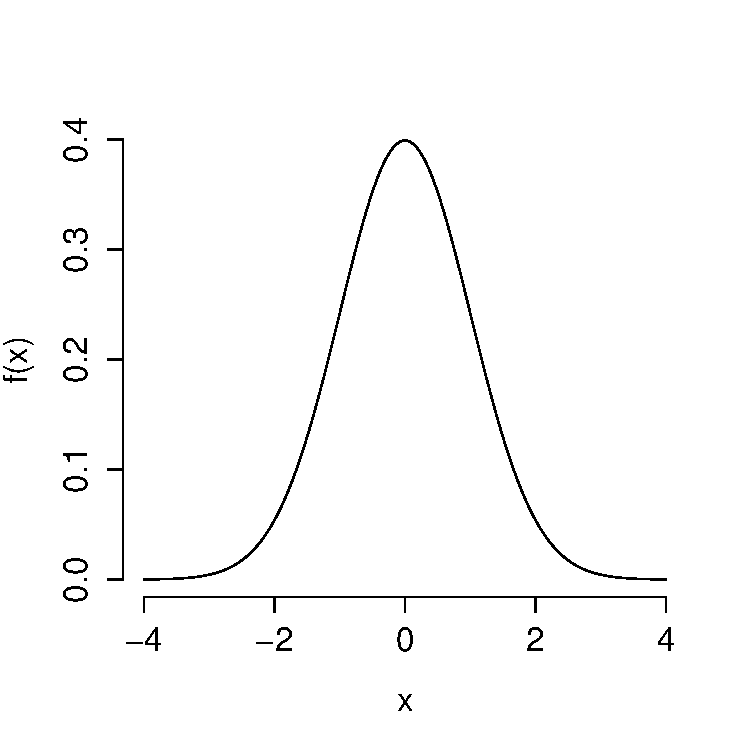
\includegraphics[scale = 0.55]{./images/tail1}
\end{center}
\end{frame}

%%%%%%%%%%%%%%%%%%%%%%%%%%%%%%%%%%%%%%%%
\begin{frame}
\frametitle{\texttt{qnorm(0.75)}$\approx 0.67$}
Suppose $X$ is a standard normal RV. What is the value of $c$ such that $P(-c \leq X\leq c ) = 0.5$?
\begin{center}
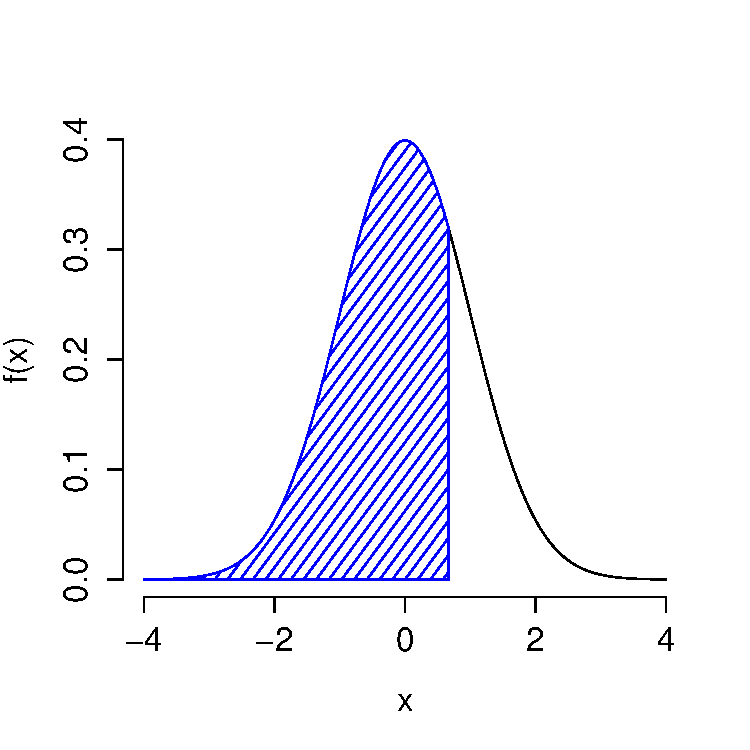
\includegraphics[scale = 0.55]{./images/tail2}
\end{center}
\end{frame}

%%%%%%%%%%%%%%%%%%%%%%%%%%%%%%%%%%%%%%%%
\begin{frame}
\frametitle{\texttt{qnorm(0.75)}$\approx 0.67$}
Suppose $X$ is a standard normal RV. What is the value of $c$ such that $P(-c \leq X\leq c ) = 0.5$?
\begin{center}
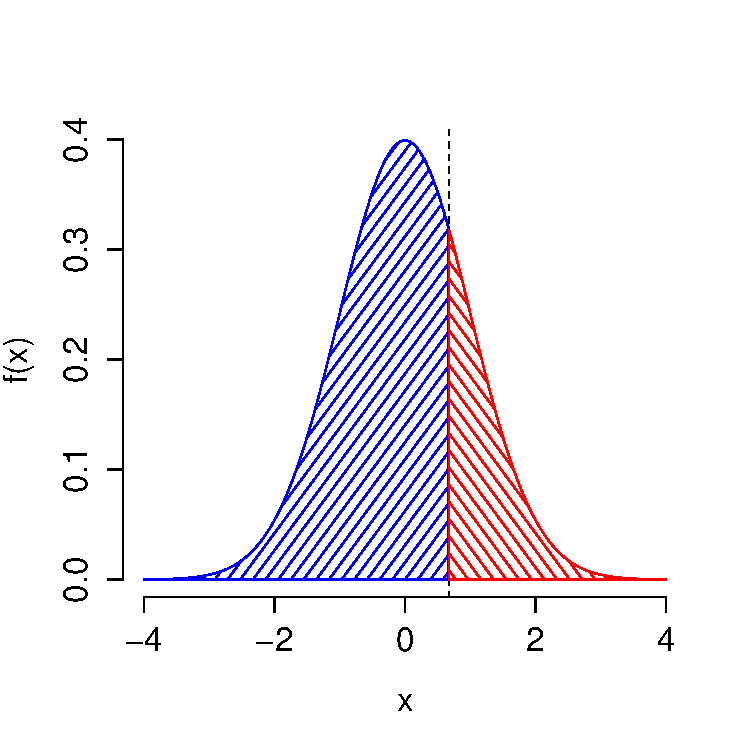
\includegraphics[scale = 0.55]{./images/tail3}
\end{center}
\end{frame}

%%%%%%%%%%%%%%%%%%%%%%%%%%%%%%%%%%%%%%%%

\begin{frame}
\frametitle{\texttt{pnorm(0.67)-pnorm(-0.67)}$\approx$?}
Suppose $X$ is a standard normal RV. What is the value of $c$ such that $P(-c \leq X\leq c ) = 0.5$?
\begin{center}
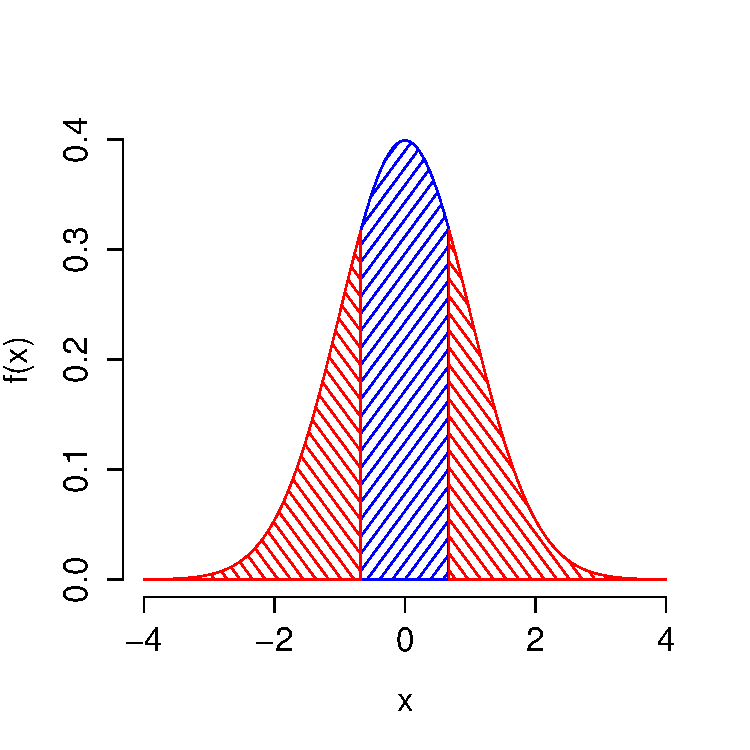
\includegraphics[scale = 0.55]{./images/tail4}
\end{center}
\end{frame}

%%%%%%%%%%%%%%%%%%%%%%%%%%%%%%%%%%%%%%%%


\begin{frame}
\frametitle{\texttt{pnorm(0.67)-pnorm(-0.67)}$\approx 0.5$}
Suppose $X$ is a standard normal RV. What is the value of $c$ such that $P(-c \leq X\leq c ) = 0.5$?
\begin{center}
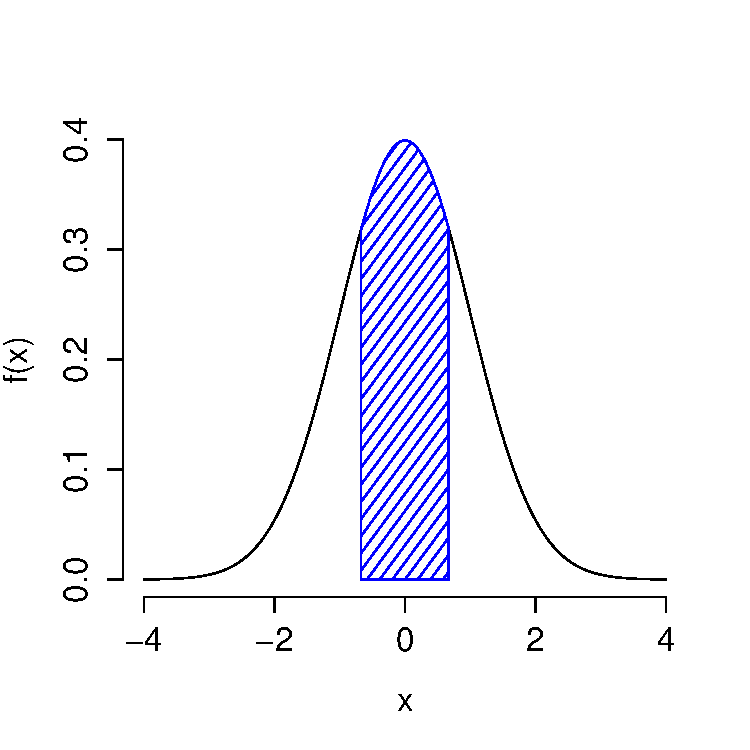
\includegraphics[scale = 0.55]{./images/tail5}
\end{center}
\end{frame}
%%%%%%%%%%%%%%%%%%%%%%%%%%%%%%%%%%%%%%%%
\begin{frame}
\frametitle{68\% Central Interval for Standard Normal \hfill 
\includegraphics[scale = 0.05]{./images/clicker}}

Suppose $X$ is a standard normal random variable. What value of $c$ ensures that $P(-c \leq X \leq c) \approx 0.68$?

\end{frame}


%%%%%%%%%%%%%%%%%%%%%%%%%%%%%%%%%%%%%%%%
\begin{frame}
\frametitle{95\% Central Interval for Standard Normal \hfill 
\includegraphics[scale = 0.05]{./images/clicker}}

Suppose $X$ is a standard normal random variable. What value of $c$ ensures that $P(-c \leq X \leq c) \approx \alert{0.95}$?

\end{frame}


%%%%%%%%%%%%%%%%%%%%%%%%%%%%%%%%%%%%%%%%

\begin{frame}
\frametitle{R Commands for \emph{Arbitrary} Normal Distributions}
Let $X \sim N(\mu, \sigma^2)$ . Then we can use R to evaluate the CDF and Quantile function of $X$ as follows:
\vspace{1em}
\begin{table}
\centering
\fbox{\begin{tabular}{ll}
CDF $F(x)$&\texttt{pnorm(x, mean = $\mu$,  sd = $\sigma$)}\\
Quantile Function $Q(p)$ & \texttt{qnorm(p, mean = $\mu$,  sd = $\sigma$)}\\
\end{tabular}}
\end{table}
\vspace{1em}
\alert{Notice that this means you don't have to transform $X$ to a standard normal in order to find areas under its pdf using R.}
\end{frame}
%%%%%%%%%%%%%%%%%%%%%%%%%%%%%%%%%%%%%%%%
\begin{frame}
\frametitle{Example from Homework: $X \sim N(0,16)$}

One Way:
			\begin{eqnarray*}
				P(X \geq 10) &=& \pause 1 - P(X \leq 10) = \pause 1 - P(X /4\leq 10/4)\\
				&=& \pause 1 - P(Z\leq 2.5) = \pause  1 - \Phi(2.5) = \pause 1 - \mbox{\texttt{pnorm(2.5)}}\\ \pause
				&\approx& 0.006
			\end{eqnarray*}
\pause
An Easier Way:
	\begin{eqnarray*}
	P(X \geq 10) &=& \pause 1 - P(X \leq 10)\\ \pause
	&=& \pause 1 - \texttt{pnorm(10, mean = 0, sd = 4)} \\ \pause
	&\approx& 0.006
	\end{eqnarray*}
\end{frame}
%%%%%%%%%%%%%%%%%%%%%%%%%%%%%%%%%%%%%%%%
\begin{frame}
Suppose $X$ has mean $\mu_x$ variance $\sigma_x^2$ and is independent of $Y$, which has mean $\mu_y$ variance $\sigma_y^2$. Let $a,b$ be constants.
\vspace{2em}

\begin{block}{What is $E[aX + bY]$?}
\pause
$E[aX + bY]=a E[X] + b E[Y] = \alert{a\mu_x + b\mu_y}$
\end{block}
\vspace{1em}

\begin{block}{What is $Var(aX + bY)$?}
\pause
$Var(aX + bY) = a^2 Var(X) + b^2 Var(Y) = \alert{a^2 \sigma_x^2 + b^2 \sigma_y^2}$
\\\alert{By independence.}
\end{block}

\end{frame}
%%%%%%%%%%%%%%%%%%%%%%%%%%%%%%%%%%%%%%%%
\begin{frame}
Now suppose $X \sim N(\mu_x, \sigma^2_x)$ independent of $Y \sim N(\mu_y, \sigma^2_y)$. Let $a,b$ be constants.
\vspace{2em}

\begin{block}{What is $E[aX + bY]$?}
\pause
$E[aX + bY]=a E[X] + b E[Y] = \alert{a\mu_x + b\mu_y}$
\end{block}
\vspace{1em}

\begin{block}{What is $Var(aX + bY)$?}
\pause
$Var(aX + bY) = a^2 Var(X) + b^2 Var(Y) = \alert{a^2 \sigma_x^2 + b^2 \sigma_y^2}$
\\\alert{By independence.}
\end{block}
\end{frame}
%%%%%%%%%%%%%%%%%%%%%%%%%%%%%%%%%%%%%%%%
\begin{frame}
\frametitle{Here's the Surprising Thing:}
\alert{If $X$ and $Y$ are independent Normal Random Variables and $a,b$ are constants, then $aX + bY$ is \emph{also} a Normal Random Variable!}
\end{frame}
%%%%%%%%%%%%%%%%%%%%%%%%%%%%%%%%%%%%%%%%
\begin{frame}
\frametitle{Linear Combinations of Independent Normals}
Let $X \sim N(\mu_x, \sigma^2_x)$ independent of $Y \sim N(\mu_y, \sigma^2_y)$. Then if $a,b,c$ are constants:

$$\boxed{aX + bY +c \sim N(a\mu_x + b\mu_y + c, a^2 \sigma_x^2 + b^2 \sigma_y^2)}$$



\begin{block}{Important}
	\begin{itemize}
		\item Result assumes independence
		\item Particular to Normal Distribution
		\item Extends to more than two Normal RVs
	\end{itemize}
\end{block}

\end{frame}
%%%%%%%%%%%%%%%%%%%%%%%%%%%%%%%%%%%%%%%%
\begin{frame}
\frametitle{Suppose $X_1, X_2, \sim \mbox{iid } N(\mu, \sigma^2)$ \hfill 
\includegraphics[scale = 0.05]{./images/clicker}}

Let $\bar{X} = (X_1 + X_2)/2$. What is the distribution of $\bar{X}$?
\begin{enumerate}[(a)]
\item $N(\mu, \sigma^2/2)$
\item $N(0,1)$
\item $N(\mu, \sigma^2)$
\item $N(\mu, 2\sigma^2)$
\item $N(2\mu, 2\sigma^2)$
\end{enumerate}

\end{frame}
%%%%%%%%%%%%%%%%%%%%%%%%%%%%%%%%%%%%%%%%
\begin{frame}
\begin{figure}
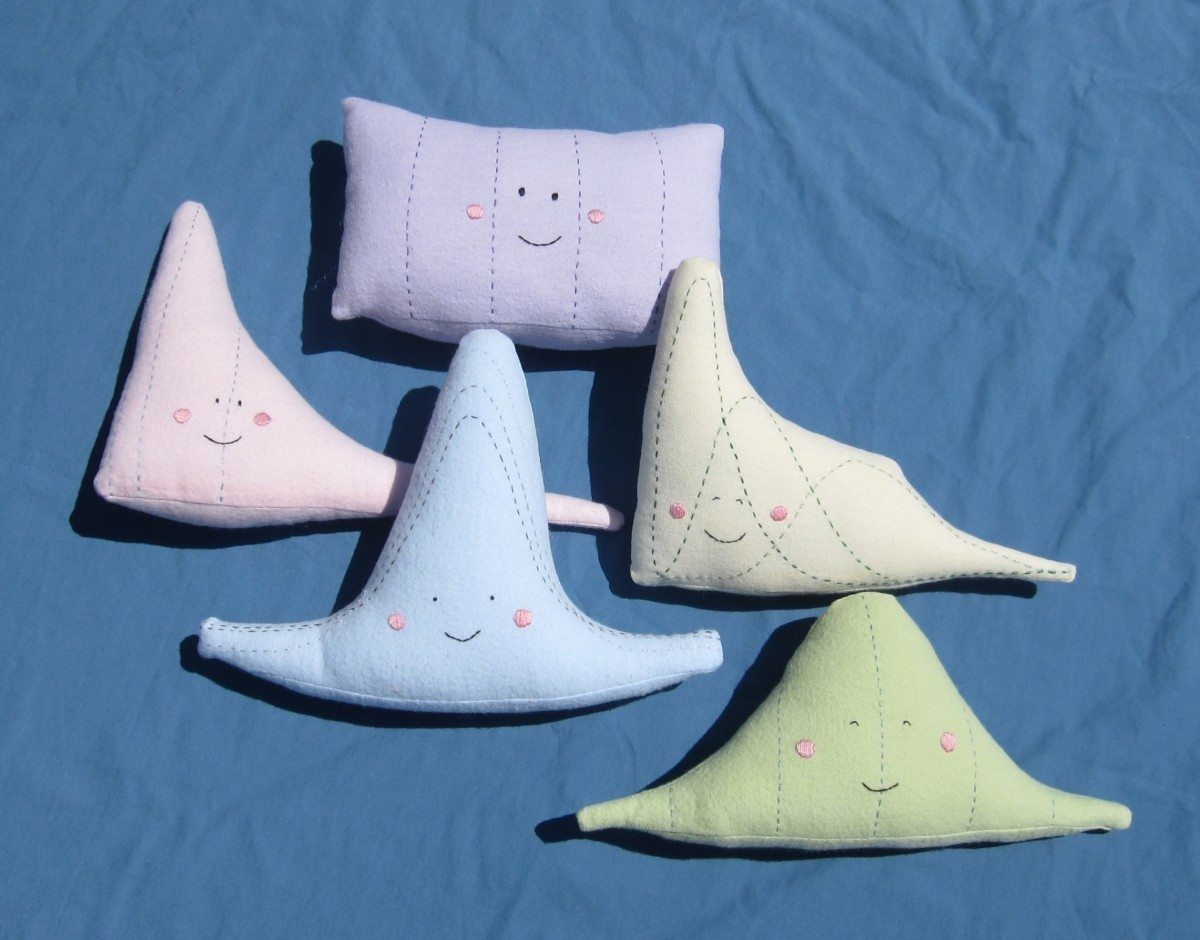
\includegraphics[scale = 0.2]{./images/normal_friends}
\caption{The Normal Distribution and Friends.}
\end{figure}
\end{frame}
%%%%%%%%%%%%%%%%%%%%%%%%%%%%%%%%%%%%%%%%
\begin{frame}
\frametitle{Functions of Independent RVs are Independent}

If $X$ and $Y$ are independent random variables and $g$ and $h$ are functions, then the random variables $g(X)$ and $h(Y)$ are also independent.

\end{frame}



%%%%%%%%%%%%%%%%%%%%%%%%%%%%%%%%%%%%%%%%
\begin{frame}
\begin{figure}
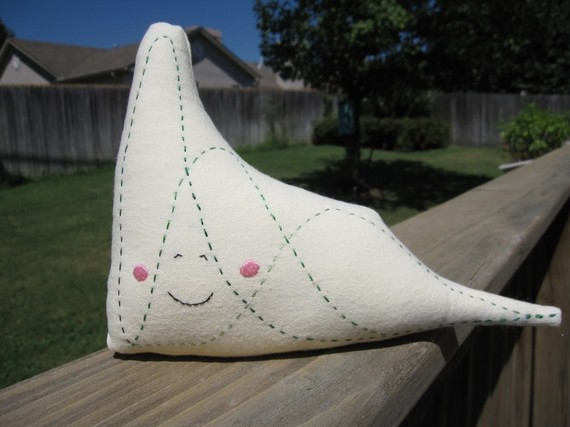
\includegraphics[scale = 0.45]{./images/chisq_etsy1}
\caption{PDF for $\chi^2$-Distribution}
\end{figure}
\end{frame}

%%%%%%%%%%%%%%%%%%%%%%%%%%%%%%%%%%%%%%%%
\begin{frame}
\begin{figure}
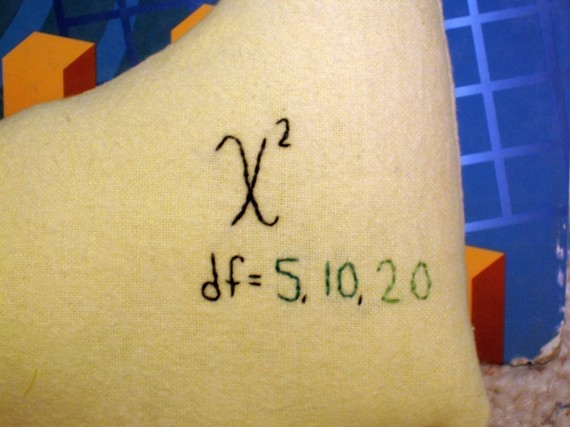
\includegraphics[scale = 0.45]{./images/chisq_etsy2}
\end{figure}
\end{frame}
%%%%%%%%%%%%%%%%%%%%%%%%%%%%%%%%%%%%%%%%
\begin{frame}
\frametitle{$\chi^2$ Random Variable}
Let $X_1, \hdots, X_\nu \sim \mbox{iid } N(0,1)$. Then,
	$$\left(X_1^2 + \hdots + X_\nu^2  \right)\sim \chi^2(\nu)$$
	where the parameter $\nu$ is the \emph{degrees of freedom}
	
	\vspace{1em}
	\pause
	\alert{Support = $(0, \infty)$}\\
	\vspace{1em}
\end{frame}




%%%%%%%%%%%%%%%%%%%%%%%%%%%%%%%%%%%%%%%%

\begin{frame}
\frametitle{$\chi^2$ PDFs}

\begin{figure}
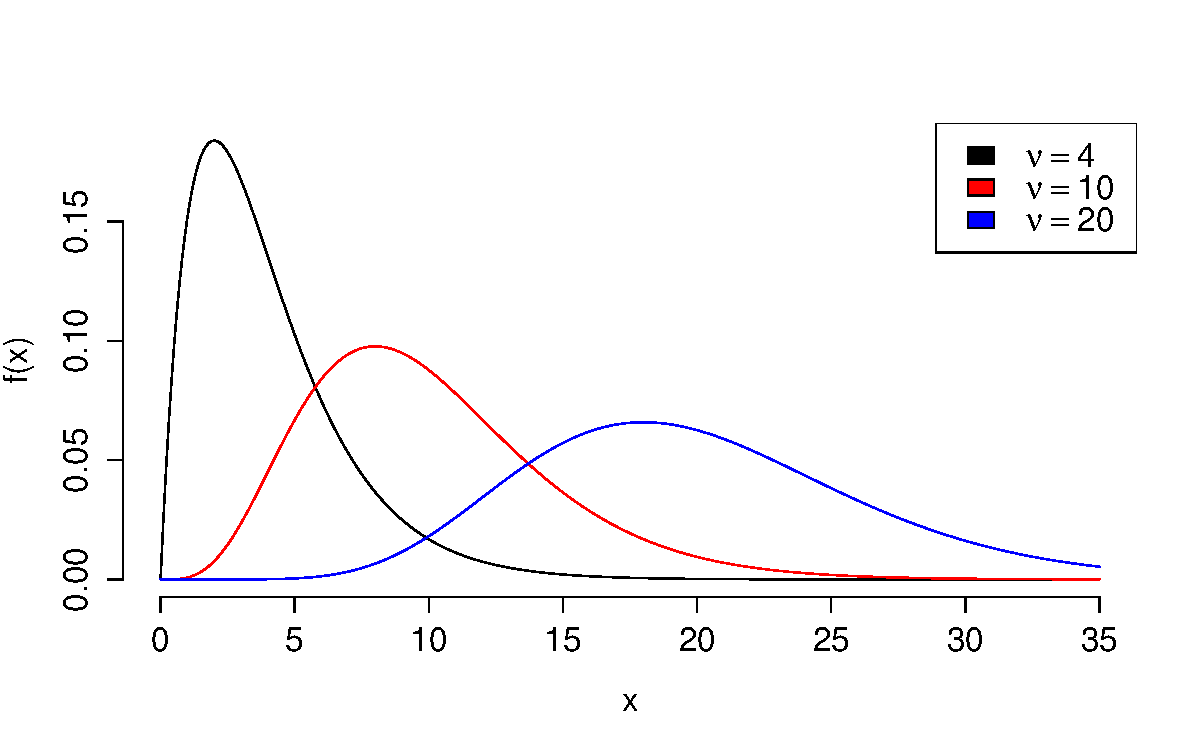
\includegraphics[scale = 0.58]{./images/chisq}
\end{figure}
\end{frame}

%%%%%%%%%%%%%%%%%%%%%%%%%%%%%%%%%%%%%%%%
%\begin{frame}
%\begin{figure}
%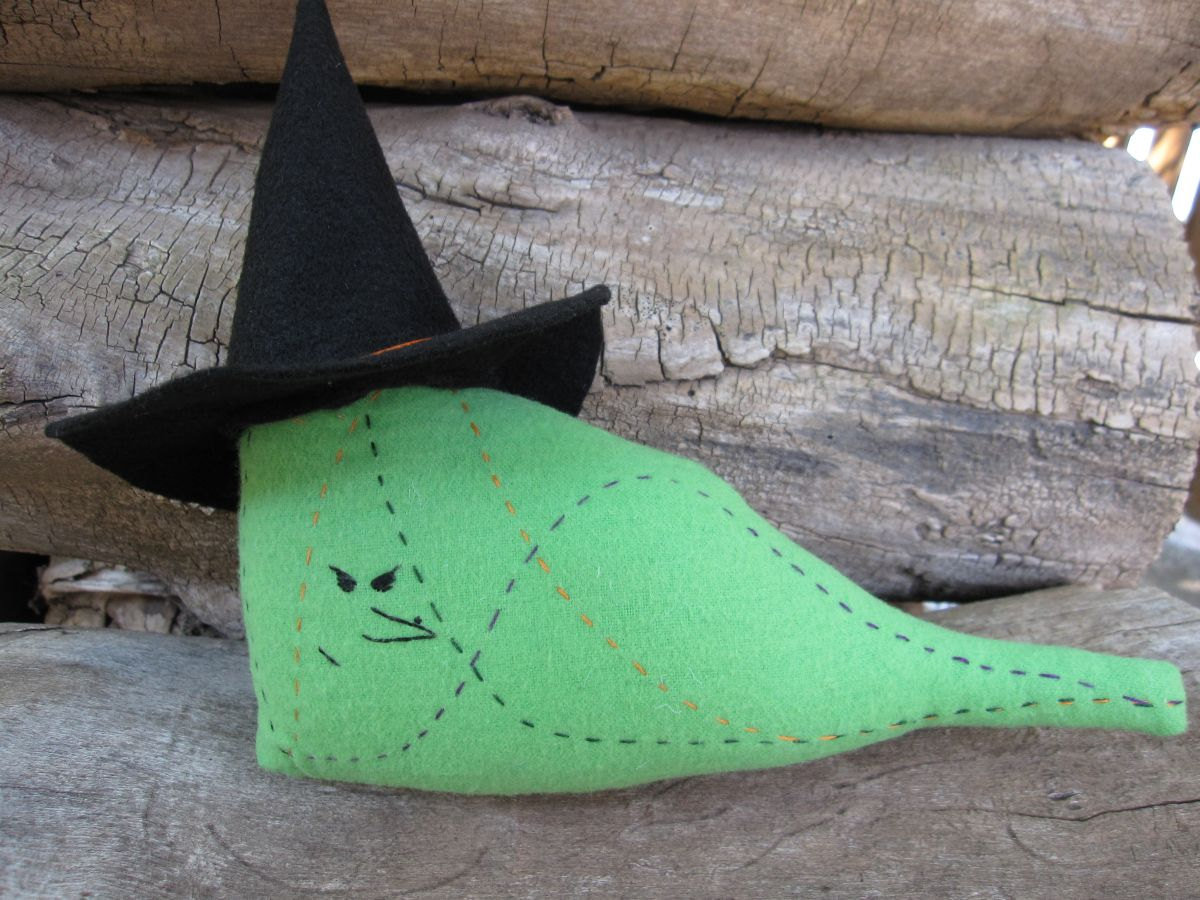
\includegraphics[scale = 0.45]{./images/chisq_etsy_witch}
%\caption{$\chi^2$ PDF -- Halloween Edition}
%\end{figure}
%\end{frame}
%%%%%%%%%%%%%%%%%%%%%%%%%%%%%%%%%%%%%%%%

\begin{frame}
\begin{figure}
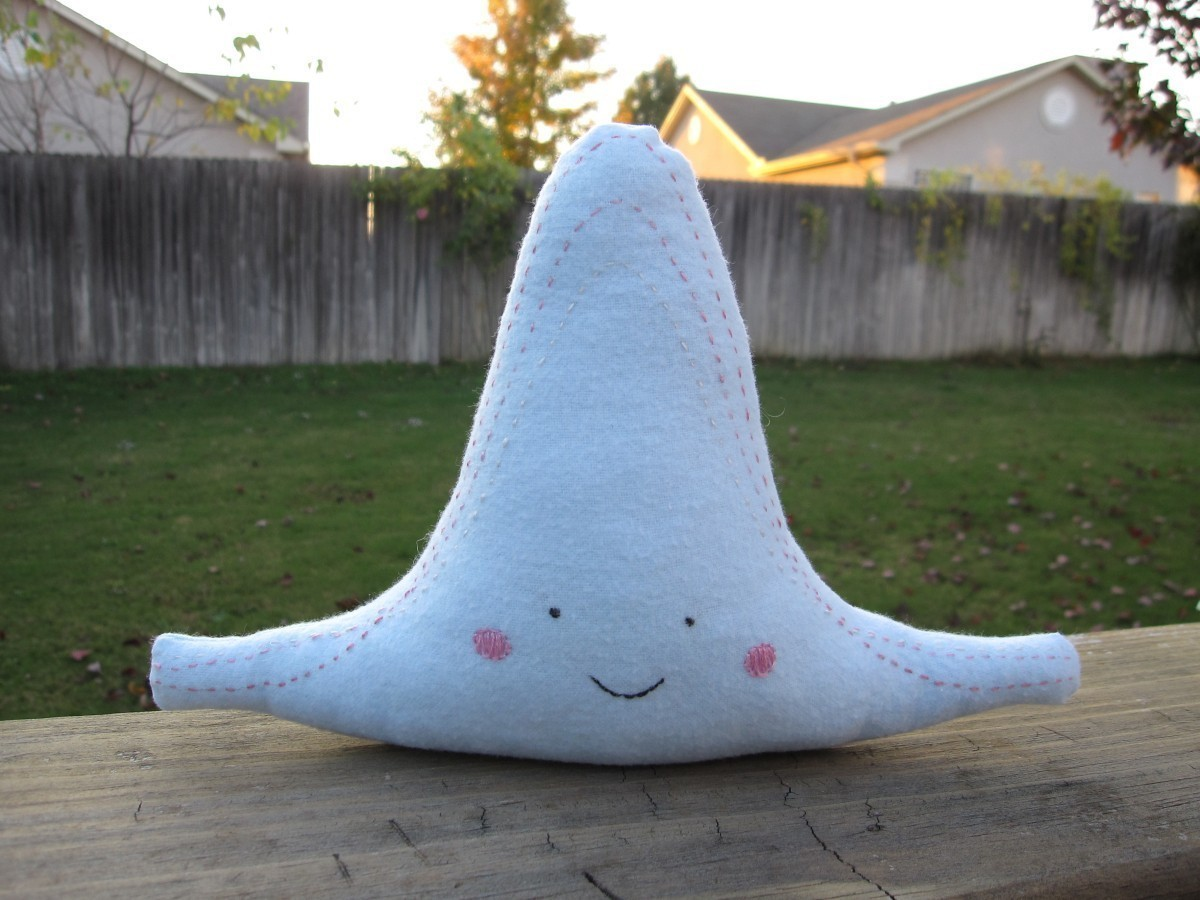
\includegraphics[scale = 0.2]{./images/t_etsy1}
\caption{PDF for Student-t Distribution}
\end{figure}
\end{frame}

%%%%%%%%%%%%%%%%%%%%%%%%%%%%%%%%%%%%%%%%
\begin{frame}
\begin{figure}
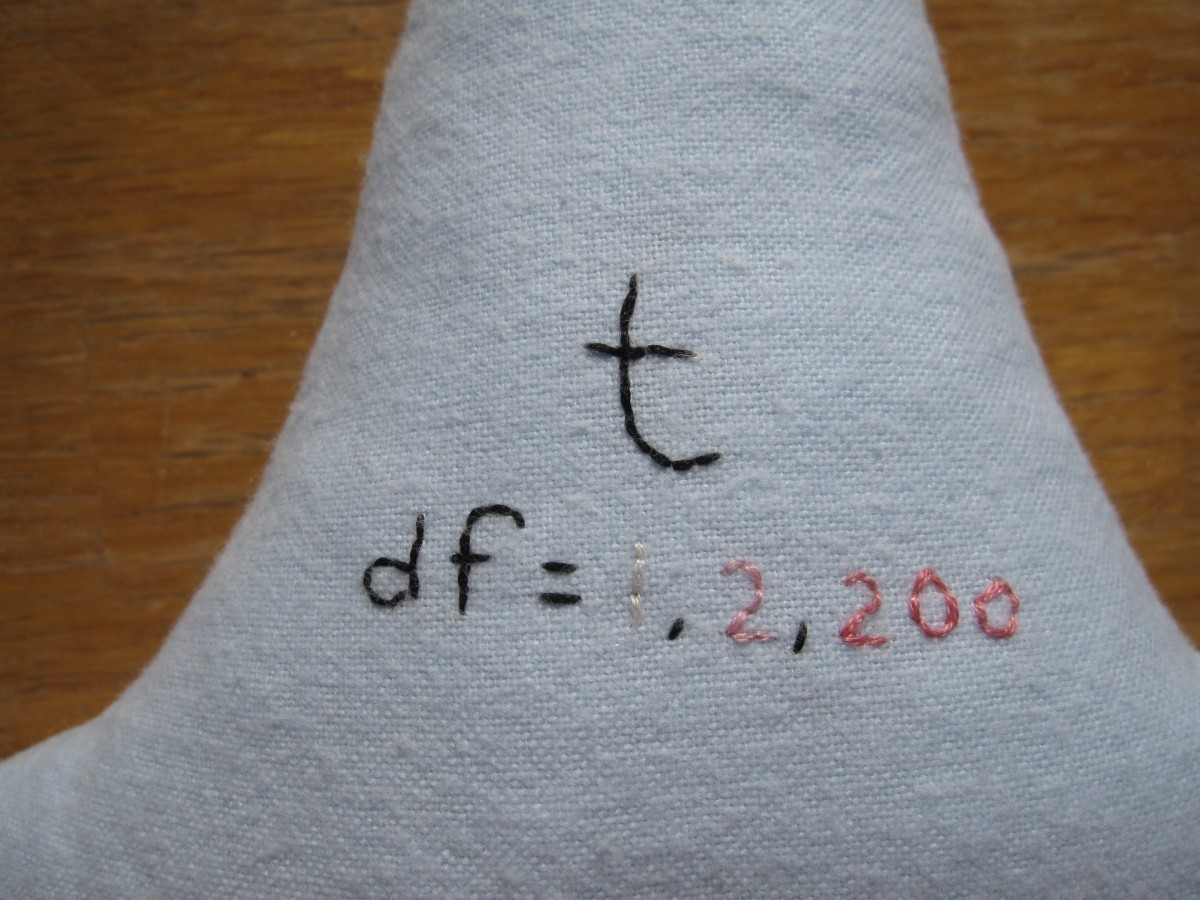
\includegraphics[scale = 0.2]{./images/t_etsy2}
\end{figure}
\end{frame}

%%%%%%%%%%%%%%%%%%%%%%%%%%%%%%%%%%%%%%%%

\begin{frame}
\frametitle{Student-t Random Variable}
Let $X \sim N(0,1)$ independent of $Y \sim \chi^2(\nu)$. Then,
$$\frac{X}{\sqrt{Y/\nu}}\sim t(\nu)$$
where the parameter $\nu$ is the degrees of freedom.

\vspace{1em}

\alert{Support = $(-\infty, \infty)$}

\vspace{1em}

\alert{As $\nu \rightarrow \infty$, $t \rightarrow$ Standard Normal.}\\
\vspace{2em}

\alert{Student-t Distribution is always symmetric and centered at zero, but mean and variance may  not exist. Degrees of freedom ($\nu$) control thickness of tails.}
\end{frame}



%%%%%%%%%%%%%%%%%%%%%%%%%%%%%%%%%%%%%%%%
\begin{frame}
\frametitle{Student-t PDFs}

\begin{figure}
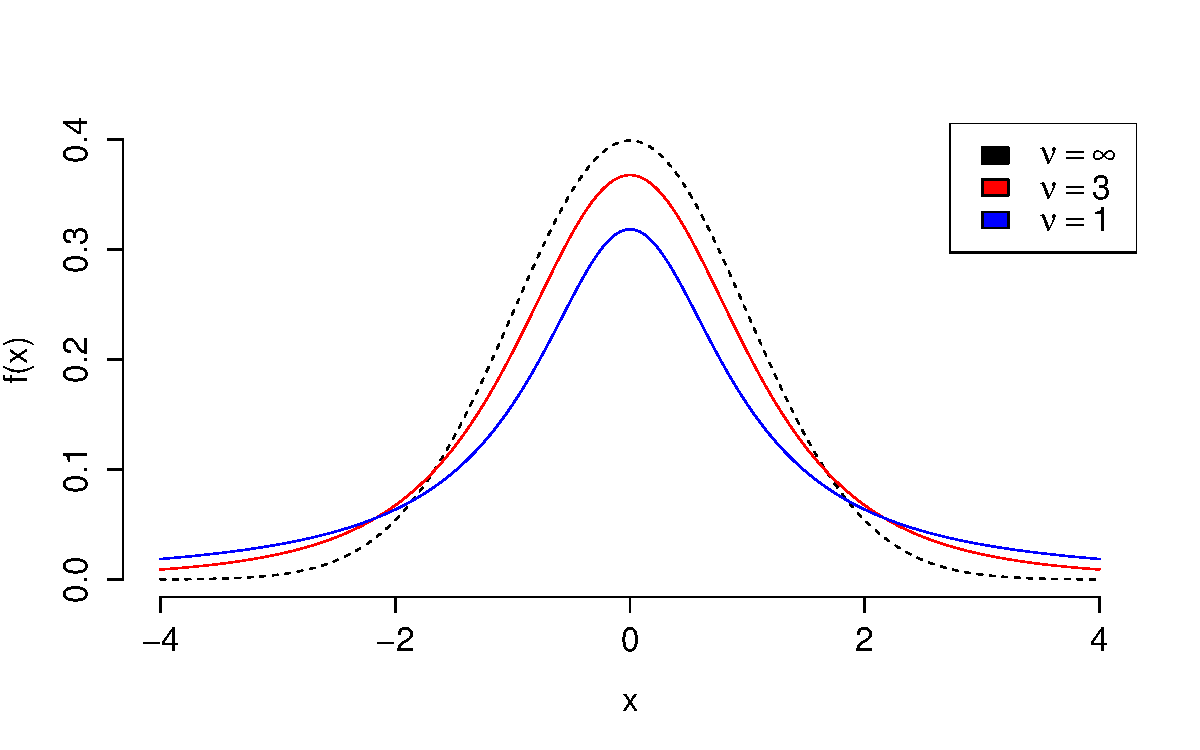
\includegraphics[scale = 0.58]{./images/tpdf}
\end{figure}
\end{frame}

%%%%%%%%%%%%%%%%%%%%%%%%%%%%%%%%%%%%%%%%
\begin{frame}
\frametitle{F Random Variable}
Suppose $X \sim \chi^2(\nu)$ independent of $Y \sim \chi^2(\omega)$. Then,
	$$\frac{X/\nu}{Y/\omega} \sim F(\nu, \omega)$$
where $\nu$ is the numerator degrees of freedom and $\omega$ is the denominator degrees of freedom.
\vspace{1em}

\pause
\alert{Support = $(0, \infty)$}\\

\end{frame}




%%%%%%%%%%%%%%%%%%%%%%%%%%%%%%%%%%%%%%%%
\begin{frame}
\frametitle{F PDFs}

\begin{figure}
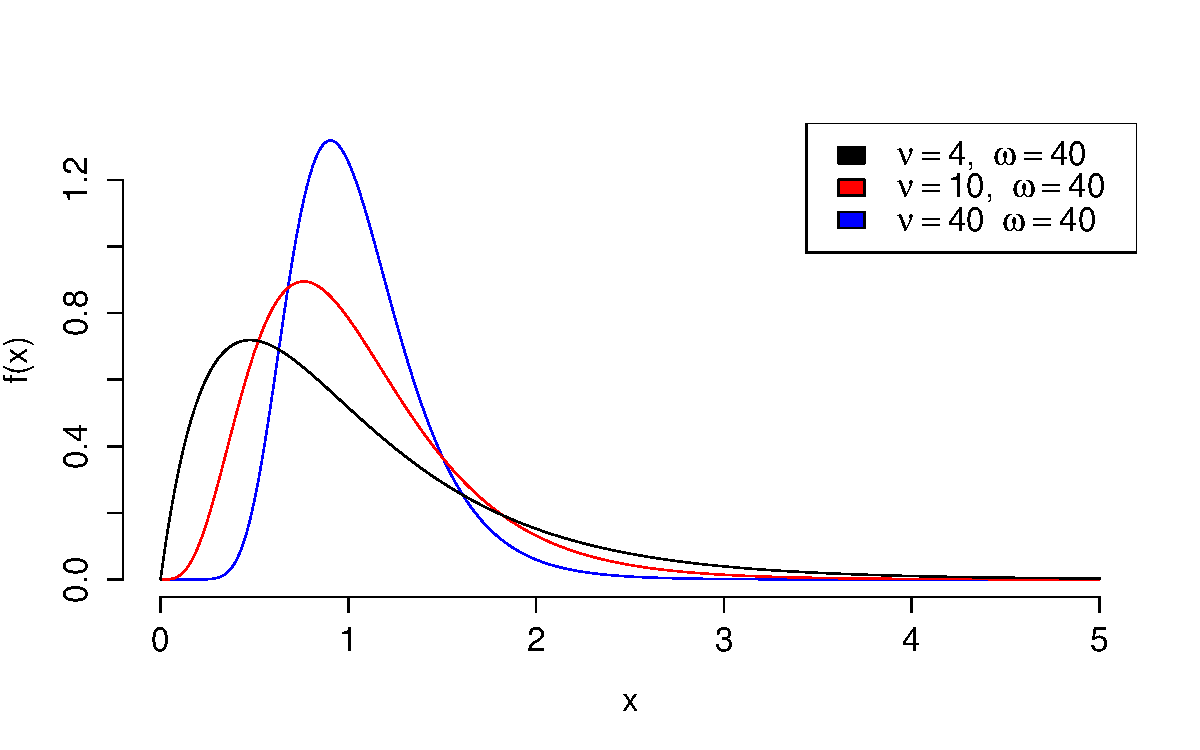
\includegraphics[scale = 0.58]{./images/Fdist}
\end{figure}
\end{frame}

%%%%%%%%%%%%%%%%%%%%%%%%%%%%%%%%%%%%%%%%

\begin{frame}
\frametitle{R Commands -- CDFs and Quantile Functions}
$F(x) = P(X\leq x)$ is the CDF, $Q(p) = F^{-1}(p)$ the Quantile Function
\footnotesize
\begin{table}
\begin{tabular}{l|ll}
&$F(x)$&$Q(p)$\\
\hline
$N(\mu,\sigma^2)$ &\texttt{pnorm(x, mean = $\mu$,  sd = $\sigma$)}&\texttt{qnorm(p, mean = $\mu$,  sd = $\sigma$)}\\
$\chi^2(\nu)$&\texttt{pchisq(x, df = $\nu$)}&\texttt{qchisq(p, df = $\nu$)}\\
$t(\nu)$&\texttt{pt(x, df = $\nu$)}&\texttt{qt(p, df = $\nu$)}\\
$F(\nu,\omega)$&\texttt{pf(x, df1 = $\nu$, df2 = $\omega$)}&\texttt{qf(p, df1 = $\nu$, df2 = $\omega$)}
\end{tabular}
\end{table}
\vspace{1em}
\normalsize
\alert{Mnemonic: ``p'' is for Probability, ``q'' is for Quantile.}

\end{frame}
%%%%%%%%%%%%%%%%%%%%%%%%%%%%%%%%%%%%%%%%
\begin{frame}
	\frametitle{\href{http://www.ditraglia.com/econ103/friends_of_normal.html}{http://www.ditraglia.com/econ103/friends\_of\_normal.html}}
\framesubtitle{Source Code on my \href{https://gist.github.com/fditraglia/7121684}{\fbox{Github Page}}}



\begin{figure}
	\fbox{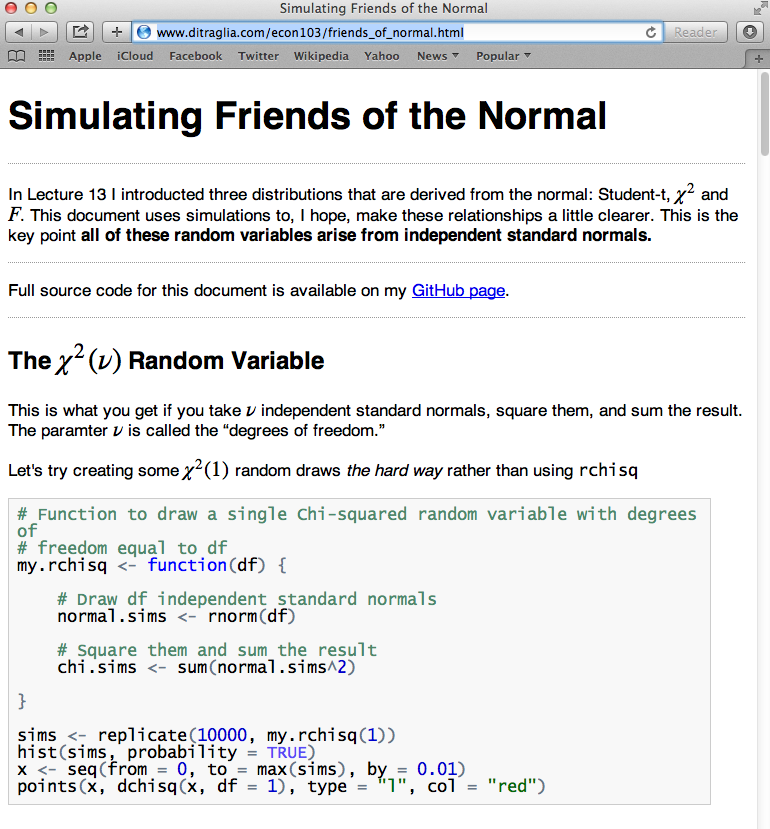
\includegraphics[scale = 0.2]{./images/normal_friends_screenshot}}
\end{figure}

\end{frame}


%%%%%%%%%%%%%%%%%%%%%%%%%%%%%%%%%%%%%%%%
\begin{frame}
\frametitle{R Commands -- PDFs and Random Draws}
\footnotesize
\begin{table}
\begin{tabular}{l|ll}
&$f(x)$&Make \texttt{n} iid Random Draws\\
\hline
$N(\mu,\sigma^2)$ &\texttt{dnorm(x, mean = $\mu$,  sd = $\sigma$)}&\texttt{rnorm(n, mean = $\mu$,  sd = $\sigma$)}\\
$\chi^2(\nu)$&\texttt{dchisq(x, df = $\nu$)}&\texttt{rchisq(n, df = $\nu$)}\\
$t(\nu)$&\texttt{dt(x, df = $\nu$)}&\texttt{rt(n, df = $\nu$)}\\
$F(\nu,\omega)$&\texttt{df(x, df1 = $\nu$, df2 = $\omega$)}&\texttt{rf(n, df1 = $\nu$, df2 = $\omega$)}
\end{tabular}
\end{table}
\vspace{1em}
\normalsize
\alert{Mnemonic: ``d'' is for Density, ``r'' is for Random.}

\end{frame}
%%%%%%%%%%%%%%%%%%%%%%%%%%%%%%%%%%%%%%%%


\begin{frame}
\frametitle{Example: $X_1, X_2, X_3 \sim \mbox{iid } N(0, 1)$}
\begin{block}{What is the distribution of $Y_1 = X_1^2 + X_2^2$?}\pause
Sum of squares of two indep.\ std.\ normals $\Rightarrow \alert{Y_1 \sim \chi^2(2)}$
\end{block}
\pause
\begin{block}{What is the distribution of $Y_2 = (Y_1/2)/(X_3^2)$?}
\pause
$Y_1 \sim \chi^2(2)$ and $X_3^2 \sim \chi^2(1)$\\
\pause
\vspace{1em}
Hence $Y_2 =$ ratio of two indep.\ $\chi^2$ RVs, each divided by its degrees of freedom $\Rightarrow \alert{Y_2 \sim F(2,1)}$
\end{block}
\pause
\begin{block}{What is the distribution of $Z = X_3/\sqrt{Y_1/2}$?}
\pause
Ratio of standard normal and square root of independent $\chi^2$ RV divided by its degrees of freedom $\Rightarrow \alert{Z \sim t(2)}$
\end{block}
\end{frame}
%%%%%%%%%%%%%%%%%%%%%%%%%%%%%%%%%%%%%%%%
\begin{frame}
\frametitle{Suppose $X_1, X_2, \sim \mbox{iid } N(\mu, \sigma^2)$ \hfill 
\includegraphics[scale = 0.05]{./images/clicker}}
Let $Y = \left( X_1 - \mu\right)^2 + \left( X_2 - \mu\right)^2$. What is the distribution of $Y/\sigma^2$?

\begin{enumerate}[(a)]
	\item $F(2,1)$
	\item $\chi^2(2)$
	\item $t(2)$
	\item $N(\mu, \sigma)$
	\item None of the above
\end{enumerate}

\end{frame}
%%%%%%%%%%%%%%%%%%%%%%%%%%%%%%%%%%%%%%%%
\begin{frame}
\frametitle{$Y_1 \sim \chi^2(2),\;\;\;\; Y_2 \sim F(2,1),\;\;\;\; Z \sim t(2)$}
\begin{block}{What is the median of $Y_1$?}
\pause
\texttt{qchisq(0.5, df = 2)}$\approx 1.4$
\end{block}
\pause
\begin{block}{What is $P(Y_2 \leq 5)$?}
\pause
\texttt{pf(5, df1 = 2, df2 = 1)}$\approx 0.7$
\end{block}
\pause
\begin{block}{What value of $c$ gives $P(-c\leq Z \leq c) = 0.5$?}
Use Symmetry (like normal) \\
$c=$\texttt{qt(0.75, df = 2)}$\approx 0.8$ 
\pause
\\or equivalently $-c =$\texttt{qt(0.25, df = 2)}$\approx -0.8$
\end{block}

\end{frame}
%%%%%%%%%%%%%%%%%%%%%%%%%%%%%%%%%%%%%%%%

\end{document}
